\chapter{Travaux effectués au CHU de Lille}

Cette section, bien que légèrement en marge du reste du rapport, a pour objectif de présenter un bref aperçu 
de plusieurs projets réalisés durant la seconde moitié de ce stage, au sein de l'équipe bioinformatique du \gls{chu}, 
principalement en lien avec le \gls{mm}. Ces projets portent essentiellement sur la gestion des pipelines d'analyse 
des données de séquençage, comprenant la création d'un nouveau pipeline, l'ajout d'une fonctionnalité spécifique à 
un pipeline existant, ainsi que la mise à jour et la rédaction de tests pour trois autres pipelines. Parallèlement, 
la gestion des cycles de qualification et de production a été assurée. Cette section a été encadrée par Augustin Boudry du \gls{chu}.

\section{Architecture logicielle et environnement utilisateur}

L'environnement de développement du \gls{chu} s'appuie sur plusieurs composantes clés, côté développeur comme côté utilisateur.
Des machines virtuelles sous Rocky Linux 9.2 sont mises à disposition pour les développements et la routine d'analyse.
Elles sont hébergées sur un \gls{hpc} orchestré via \href{https://oar.imag.fr/}{OAR} et très récemment \href{https://slurm.schedmd.com/documentation.html}{Slurm},  
comprenant X Go de mémoire vive, X nœuds de calcul, deux serveurs GPU, ainsi qu'un serveur de stockage de X To.
Le gestionnaire de \textit{workflow} \href{https://www.nextflow.io/}{Nextflow} est utilisé pour l'écriture des différents pipelines d'analyse, 
déployés via une conteneurisation des dépendances dans des images \textit{Singularity} et de l'environnement dans des conteneurs \textit{Docker}.
De nombreuses surcouches logicielles sont développées par l'équipe afin de faciliter, automatiser et sécuriser les phases de développement et d'utilisation.
On peut citer notamment les \textit{nf-tools}, qui permettent d'automatiser un certain nombre de tâches, allant de la création des projets au lancement des pipelines.
Enfin, des interfaces web permettent d'accéder de façon simple à l'ensemble des applications développées par l'équipe (\autoref{fig:bioinfo-dashboard}).
L'ensemble du code est versionné et hébergé sur un dépôt GitLab interne au \gls{chu}.

schéma Augustin architecture ? 

\begin{figure}[H]
    \centering
    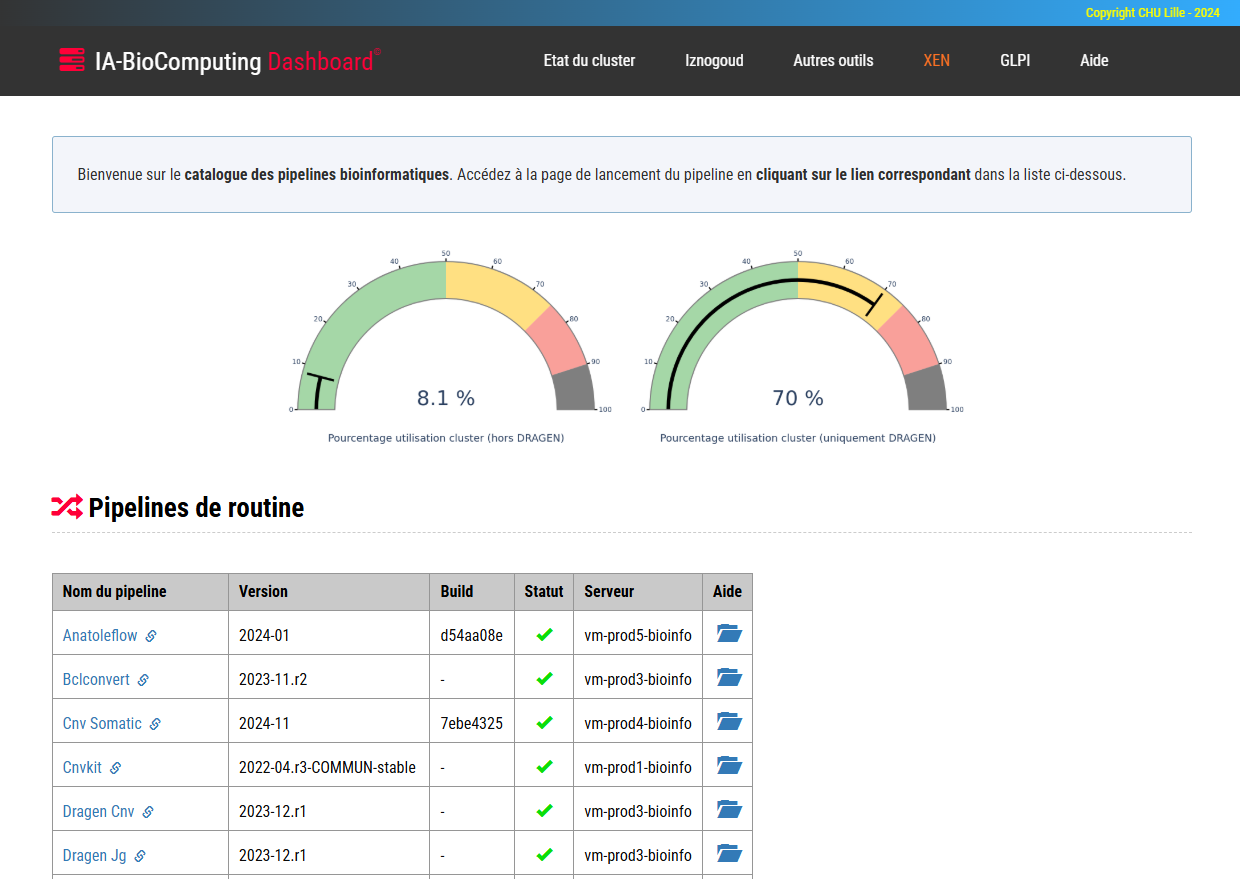
\includegraphics[width=1\textwidth]{images/dashboard_bioinfo.png}
    \caption{
        Page d'acceuil de lancement des pipelines et autres outils bioinformatiques du \gls{chu}.
    }
    \label{fig:bioinfo-dashboard}
\end{figure}

\section{Quantification des délétions du gène \textit{TP53}}

Ce rapport a principalement traité du suivi de la \gls{mrd} dans le \gls{mm}, une analyse à visée pronostique réalisée au cours du suivi des patients.
Plaçons-nous à présent dans une optique toujours pronostique (voire diagnostique) mais cette fois au moment du diagnostic de la pathologie. 
Trois analyses moléculaires sont alors réalisées :

\begin{itemize}
    \item \textbf{La recherche de variants somatiques} dans des gènes d'intérêt, notamment des oncogènes et des gènes suppresseurs de tumeurs.
    \item \textbf{La recherche de translocations} impliquant les \glspl{ig} et d'autres partenaires chromosomiques.
    \item \textbf{L'analyse du nombre de copies} permettant d'identifier des anomalies comme des duplications ou des délétions.
\end{itemize}

\vspace{1em}

C'est dans le cadre de cette dernière analyse qu'il a été nécessaire de développer une approche spécifique pour quantifier les délétions du gène \textit{TP53}, 
gène suppresseur de tumeur dont l'altération est associée à un mauvais pronostic dans le \gls{mm}, avec un seuil placé à 20 \% des cellules selon des recommandations 
récentes non publiées \cite{flyntPrognosisBiologyTargeting2020}.
Les plasmocytes étant des cellules particulièrement difficiles à cultiver, l'analyse du nombre de copies, associée aux techniques de \gls{fish} 
\footnote{La \gls{fish} est une technique de cytogénétique moléculaire permettant de détecter et localiser des séquences d'ADN spécifiques sur des chromosomes, à l'aide de sondes fluorescentes complémentaires. 
Elle est couramment utilisée pour identifier des anomalies chromosomiques, telles que des translocations, délétions ou amplifications.}, constitue l'unique 
moyen d'accéder aux remaniements génomiques de grande taille (duplications, délétions, translocations, etc.).
Ces informations permettent de dresser ce que l'on peut considérer comme un « carytoype moléculaire » de la cellule tumorale. 

\vspace{1em}

Il est aisé, grâce à la technique de \gls{fish}, de quantifier ce type d'événement en comptant directement le nombre de cellules portant l'anomalie parmi l'ensemble des cellules analysées 
(\autoref{fig:fish}).  
En revanche, il est beaucoup plus difficile d'estimer avec précision la fréquence de ces anomalies dans le cadre d'analyses en \textit{bulk}, comme celles réalisées par \gls{ngs}.

\begin{figure}[H]
    \begin{minipage}{0.45\textwidth}
        \centering
        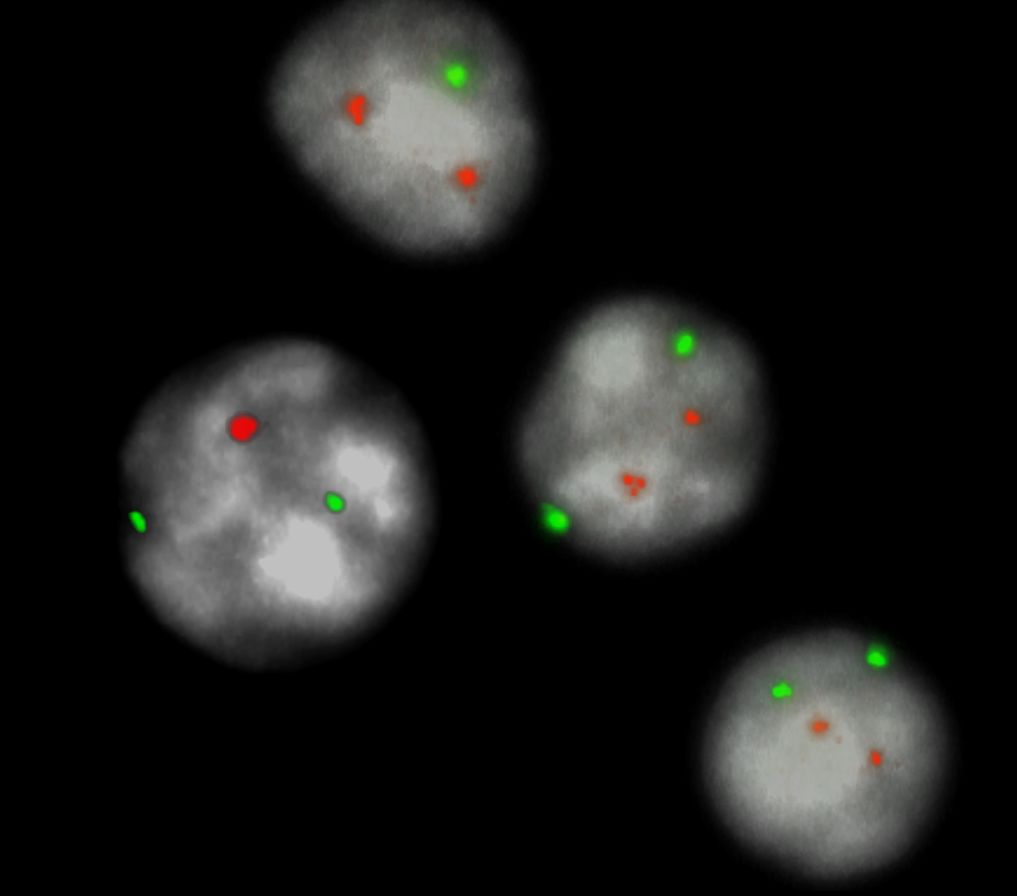
\includegraphics[width=1\textwidth]{images/fish_image.png}
    \end{minipage}
    \hfill
    \begin{minipage}{0.45\textwidth}
        \centering
        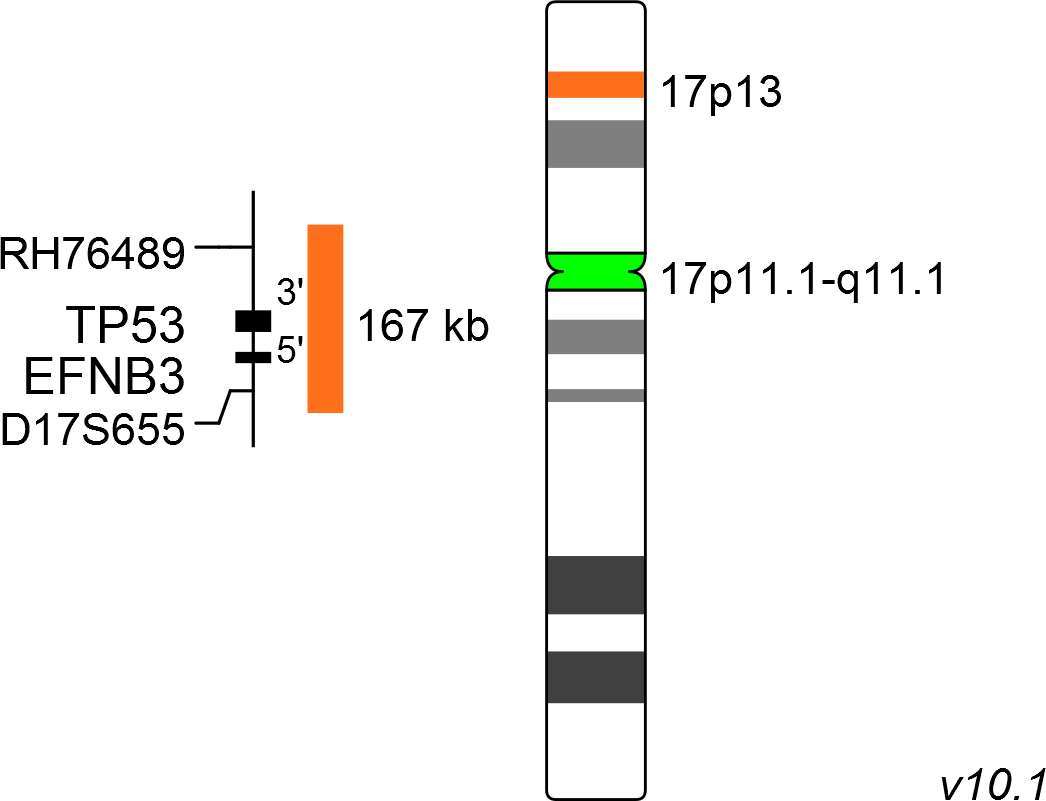
\includegraphics[width=01\textwidth]{images/fish.png}
    \end{minipage}
    \caption{
        \gls{fish} \textit{TP53} sur noyaux interphasiques à gauche et \textit{design} de la sonde à droite. 
    }
    \label{fig:fish}
\end{figure}

Pour des raisons internes au laboratoire, l'analyse par \gls{fish} n'est pas réalisable dans ce contexte.  
L'objectif a donc été de développer et d'évaluer une solution d'estimation de la fréquence des délétions de \textit{TP53} à partir des données issues du \gls{ngs}. 
L'analyse du nombre de copies repose classiquement sur le rapport des pronfondeurs sur certaines régions, et est exprimé en ratio : 1 sans anomalie, inférieur à 1 si délétion 
et supérieur à 1 si gain de la région (\autoref{fig:cnv}). Ainsi à partir de cette valeur et en posant les hypothèses suivantes :

\begin{itemize}
    \item Les délétions de \textit{TP53} sont toujours monoalléliques.
    \item L'anomalie est clonale (hypothèse non vérifiée en pratique).
    \item La pureté tumorale de l'échantillon est connue.
\end{itemize}

\begin{figure}[H]
    \centering
    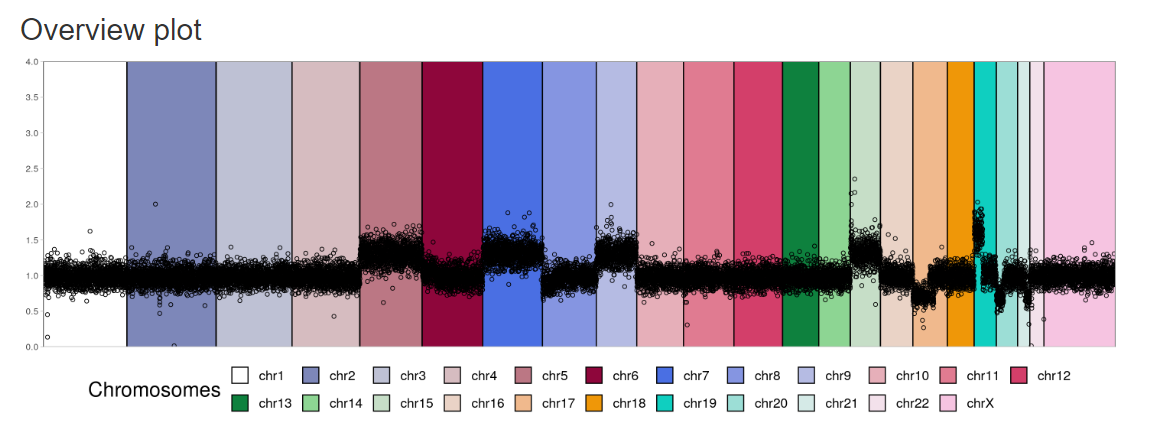
\includegraphics[width=1\textwidth]{images/cnv.png}
    \caption{Résultat de l'analyse du nombre de copies sur un échantillon de myélome multiple.}
    \label{fig:cnv}
\end{figure}

Il est alors possible de moyenner la valeur du $\log_2$ du ratio de profondeur pour les 10 sondes couvrant la région du gène \textit{TP53},  
et de l'exprimer comme une fréquence estimée de cellules délétées selon la relation suivante :

\begin{equation}
    \text{Fréquence des cellules délétées (\%)} = \left( \frac{1 - 2^{\overline{\log_2\text{Ratio}}}}{0{,}5} \right) 
    \times \frac{1}{\text{pureté}} \times 100
    \footnote{Pour exprimer le ratio de profondeur en fréquence de cellules delétées, on soustrait à 1 la valeur du ratio pour exprimer la perte relative, 
    que l'on divise par 0{,}5 qui représente la délétion monoallélique de la totatilité des cellules (une normalisation en quelque sorte). Le reste de l'expression 
    permet de corrigier par la pureté tumorale de l'échantillon, qui est le pourcentage de cellules tumorales dans l'échantillon analysé, et exprime le résultat en pourcentage.}
\end{equation}

\begin{equation}
    \text{où} \quad \overline{\log_2\text{Ratio}} = \frac{1}{n} \sum_{i=1}^{n} \log_2\text{Ratio}_i
    \footnote{Par les propriétés des logarithmes, $\overline{\log_2\text{Ratio}} = \frac{1}{n} \sum \log_2 \text{Ratio}_i = \log_2\left( \prod \text{Ratio}_i^{1/n} \right) = 
    \log_2\left( \sqrt[n]{\prod \text{Ratio}_i} \right)$, ce qui revient donc à calculer le logarithme de la moyenne géométrique.}
\end{equation}

    
Un intervalle de confiance et des statistiques de dispersion peuvent également être calculés pour évaluer la qualité de l'estimation. Cette 
approche a été implémentée dans un process \textit{Nextflow} final appelant un script Python permettant de générer au travers d'un fichier excel, 
une fréquence de délétion estimée par échantillon, et pouvant être corrigée selon la pureté tumorale (\autoref{fig:excel-tp53}). 
Par la suite l'analyse de témoins négatifs et positifs (échantillon avec ou sans délétion du gène \textit{TP53}) ont permis d'estimer 
la limite de quantification à 20 \% et de détection à 15 \% de cellules délétées.

\begin{figure}[H]
    \centering
    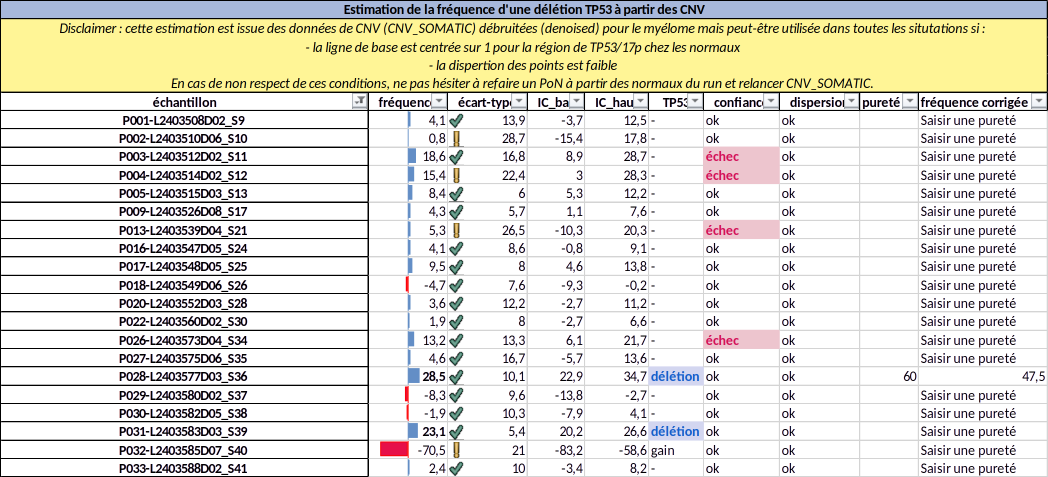
\includegraphics[width=1\textwidth]{images/excel_tp53.png}
    \caption{Résultat de l'analyse des délétions \textit{TP53} sur des échantillons de myélome multiple.}
    \label{fig:excel-tp53}
\end{figure}

\section{Seuil optimal de détection des translocations \textit{IgH}}

En lien avec la section précédente, une autre optimisation a pu être proposée concernant la recherche des translocations impliquants les \glspl{ig}.
Ces anomalies sont particulièrement importantes, considérées comme fondatrices dans l'oncogènese du \gls{mm} et leur détection se fait au \gls{chu} 
par appel de variants structuraux sur \textit{paired-end short-reads} via les \textit{caller} \textit{Manta} \cite{chenMantaRapidDetection2016a} et 
\textit{Gridss} \cite{cameronGRIDSSSensitiveSpecific2017a}. Ces deux \textit{variant-callers} fonctionnent de manière similaire en assemblant des \textit{reads} candidats
porteurs d'information structurale (\textit{split-reads}\footnote{Les \textit{split-reads} sont des lectures dont une portion s'aligne sur une région du génome 
et une autre portion sur une région distante.} et \textit{discordantly aligned reads}\footnote{Les \textit{discordantly aligned reads} 
sont des paires de lectures dont l'orientation ou la distance d'alignement est anormale par rapport à ce qui est attendu.}).

\vspace{1em}

Les résultats sont ainsi rendus sous forme de page web statique (\autoref{fig:translocation-web}), après filtrage des variants en dehors des régions d'intérêt, et en dessous d'un seuil 
de détection fixé à 10 événements supports (\textit{reads} ou paires de \textit{reads}). Des observations réalisées sur des analyses au laboratoire 
laissent à penser que certaines translocations veritables sont présentes en dessous de ce seuil fixé à 10, notamment sur des \gls{adnc}.
C'est donc concernant ce dernier, initialement fixé de manière empirique, qu'un travail d'optimisation a été entrepris afin de déterminer 
s'il permettait effectivement de discriminer de manière fiable les réarrangements pertinents des artéfacts, tout en conservant une sensibilité adéquate 
pour la détection d'événements rares. 

\begin{figure}[H]
    \centering
    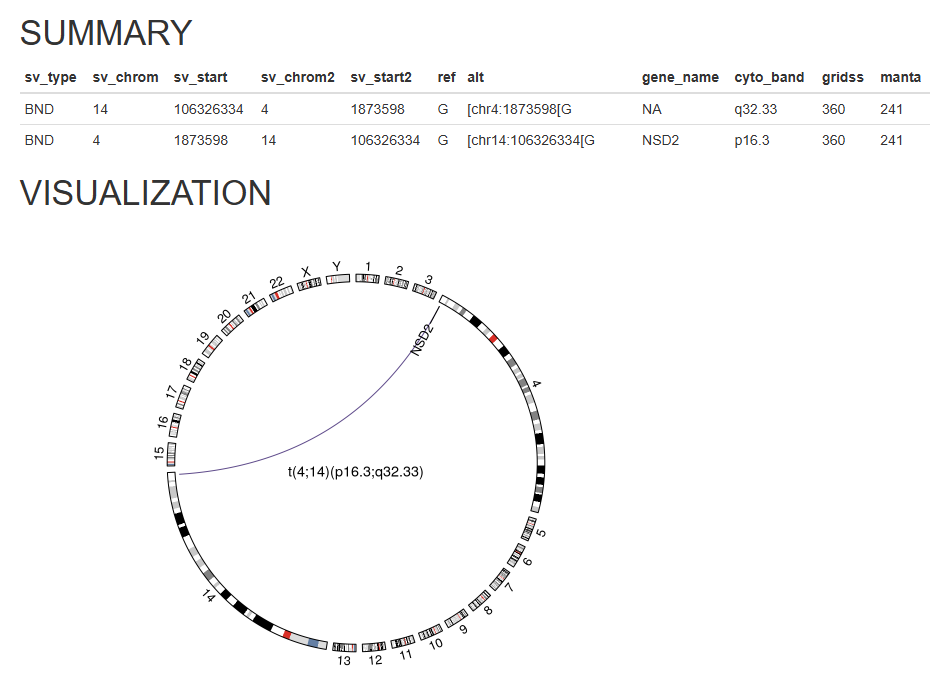
\includegraphics[width=1\textwidth]{images/translocation_web.png}
    \caption{
        Résultat de l'analyse des translocations \gls{igh} sur un échantillon de myélome multiple, 
        retrouvant ici une translocation t(4;14)(p16.3;q32.33) \textit{NSD2::IGH}.
        }
    \label{fig:translocation-web}
\end{figure}

Une manière d'aborder ce problème consiste à envisager une optimisation \textit{a posteriori}, reposant sur les nombreuses données déjà acquises, 
en formulant des hypothèses et en s'appuyant sur quelques vérités biologiques :

\begin{itemize}
    \item Les événements rapportés par \textit{Manta} et \textit{Gridss} reposent sur des signaux difficilement attribuables à des artéfacts, et peuvent donc être considérés comme fiables.
    \item Les translocations impliquant les \textit{\gls{igh}} sont des événements fondateurs, uniques et exclusifs : un patient ne présente au maximum qu'une seule translocation de ce type.
    \item À l'inverse, les translocations de type t(8;14) sont souvent secondaires, et peuvent coexister avec d'autres anomalies.
\end{itemize}

\vspace{1em}

Dans cette optique, on peut chercher à définir un seuil de détection optimisé, qui maximise le nombre de patients identifiés comme porteurs d'une translocation, 
tout en minimisant le nombre de patients présentant plusieurs anomalies, phénomène assez rare biologiquement. Ainsi on note $T$ le nombre de patients 
présentant au moins une translocation et $T_{+}$ le nombre présentant plusieurs translocations, en excluant les t(8;14). $T$ et $T_{+}$ sont alors des fonctions 
de $t$ définies sur $\mathbb{N}$ et à valeurs dans $\mathbb{N}$, $t$ désignant le seuil en dessous duquel l'anomalie n'est pas retenue. On peut donc formuler la question sous la forme d'une optimisation sous contrainte, 
où $\delta$ représente un nombre acceptable de patients présentant plusieurs translocations, et $t^*$ le seuil optimal retenu :

\begin{equation}
    t^* = \arg\max_{t} \; T(t) \quad \text{tel que} \quad T_{+}(t) \leq \delta
 \end{equation}
    
 Il est assez aisé de résoudre le problème par recherche exhaustive sur un intervalle restreint, ou graphiquement à partir des 1178 échantillons du \gls{chu} et en faisant varier 
 $t$ de $1$ à $100$ avec $\delta < 1 \%$. Ceci nous permet d'abaisser le seuil initialement à 10, à une valeur de 6 (\autoref{fig:translocation-threshold}).


\begin{figure}[H]
    \centering
    \begin{tikzpicture}
        \begin{axis}[
            width=15cm,
            height=8cm,
            xlabel={Seuil $t$},
            xmode=log,
            extra x ticks={6},
            extra x tick labels={$6$},
            ylabel={Nombre de patients},
            legend pos=north east,
            grid=major,
        ]
        \addplot[
            color=Purple,
            mark=*,
        ] table [x=t, y=T, col sep=comma] {data/threshold_analysis.csv};
        \addlegendentry{$T(t)$}

        \addplot[
            color=Goldenrod,
            mark=square*,
        ] table [x=t, y=T+, col sep=comma] {data/threshold_analysis.csv};

        \draw[dashed, thick] (axis cs:6,-100) -- (axis cs:6,1000);
        \node at (axis cs:6.5,450) [anchor=west, font=\small, text=black] {seuil $t^*$ optimal};

        \addlegendentry{$T_+(t)$}
        \end{axis}
    \end{tikzpicture}
    \caption{
        Courbes de \textcolor{Purple}{$T(t)$} et \textcolor{Goldenrod}{$T_+(t)$} à partir des 1178 échantillons du \gls{chu}.
        Le seuil optimal $t^*$ est indiqué par la ligne pointillée, il est choisi de façon à maximiser \textcolor{Purple}{$T(t)$} 
        tout en contraignant \textcolor{Goldenrod}{$T_+(t)$} en dessous de 10.
        }
    \label{fig:translocation-threshold}
\end{figure}


\section{Statistiques sur les données de \textit{Vidjil} issues du CHU de Lille}

Le dernier travail présenté dans ce rapport se situe à l'interface des deux sections précédentes. Il a consisté à réutiliser les données issues de \textit{Vidjil}, obtenues au \gls{chu}, 
afin d'établir des statistiques à grande échelle sur les résultats analysés. Deux types d'échantillons sont traités en routine : d'une part, des \glspl{lal}, pour identifier les 
réarrangements des clones tumoraux et concevoir des systèmes personnalisés de suivi de la \gls{mrd} par \gls{pcr} quantitative ; d'autre part, des \glspl{llc}, pour l'étude du taux 
d'hypermutation des gènes \textit{IGHV}. L'objectif est d'extraire et de visualiser des tendances générales à partir du volume important de données acquises.

\vspace{1em}

Le traitement des données brutes issues des analyses par \textit{Vidjil} est réalisé via un script Python (\texttt{clone.py}) qui importe les fichiers d'analyse au format \gls{json}. 
Ce script construit des objets \texttt{Vidjil} représentant chaque analyse, ainsi que des objets \texttt{Clone} extrayant les informations essentielles des clones détectés, 
telles que la taille relative, les séquences CDR3, les gènes V(D)J assignés, la productivité, etc. Une étape d'enrichissement par requête du serveur IMGT/V-QUEST 
(sans API, nécessitant donc de récupérer et traiter la page web complète) permet d'obtenir des annotations biologiques complémentaires, notamment le pourcentage d'identité des séquences V.
Par ailleurs, les métadonnées associées aux échantillons sont intégrées afin d'assurer une contextualisation clinique et biologique des résultats.

\vspace{1em}

Un second script (\texttt{process\_dir.py}) traite de manière automatisée un ensemble de fichiers d'analyse et de métadonnées situés dans un répertoire donné. 
Il agrège les informations des clones extraits selon le type d'échantillon (\gls{llc} ou \gls{lal}). Les résultats sont synthétisés dans un fichier TSV exploitable 
pour des analyses ultérieures, avec au total plus de 4000 échantillons pour 11000 clones.

\vspace{1em}

Pour finir un tableau de bord interactif a été développé à l'aide de \textit{Streamlit} (\texttt{stat\_display.py}) pour permettre l'exploration dynamique des données. 
Ce tableau de bord propose des filtres par type d'échantillon (\gls{lal}, \gls{llc} ou inconnu), par nom d'échantillon, etc. Les résultats, bien qu'intéressants, sortent du cadre 
de ce rapport ne traitant pas de la même pathologie et ne seront pas présentés ici, mais en voici une illustration pour le plaisir des yeux (\autoref{fig:vidjil-stat}) :

\begin{figure}[H]
    \centering
    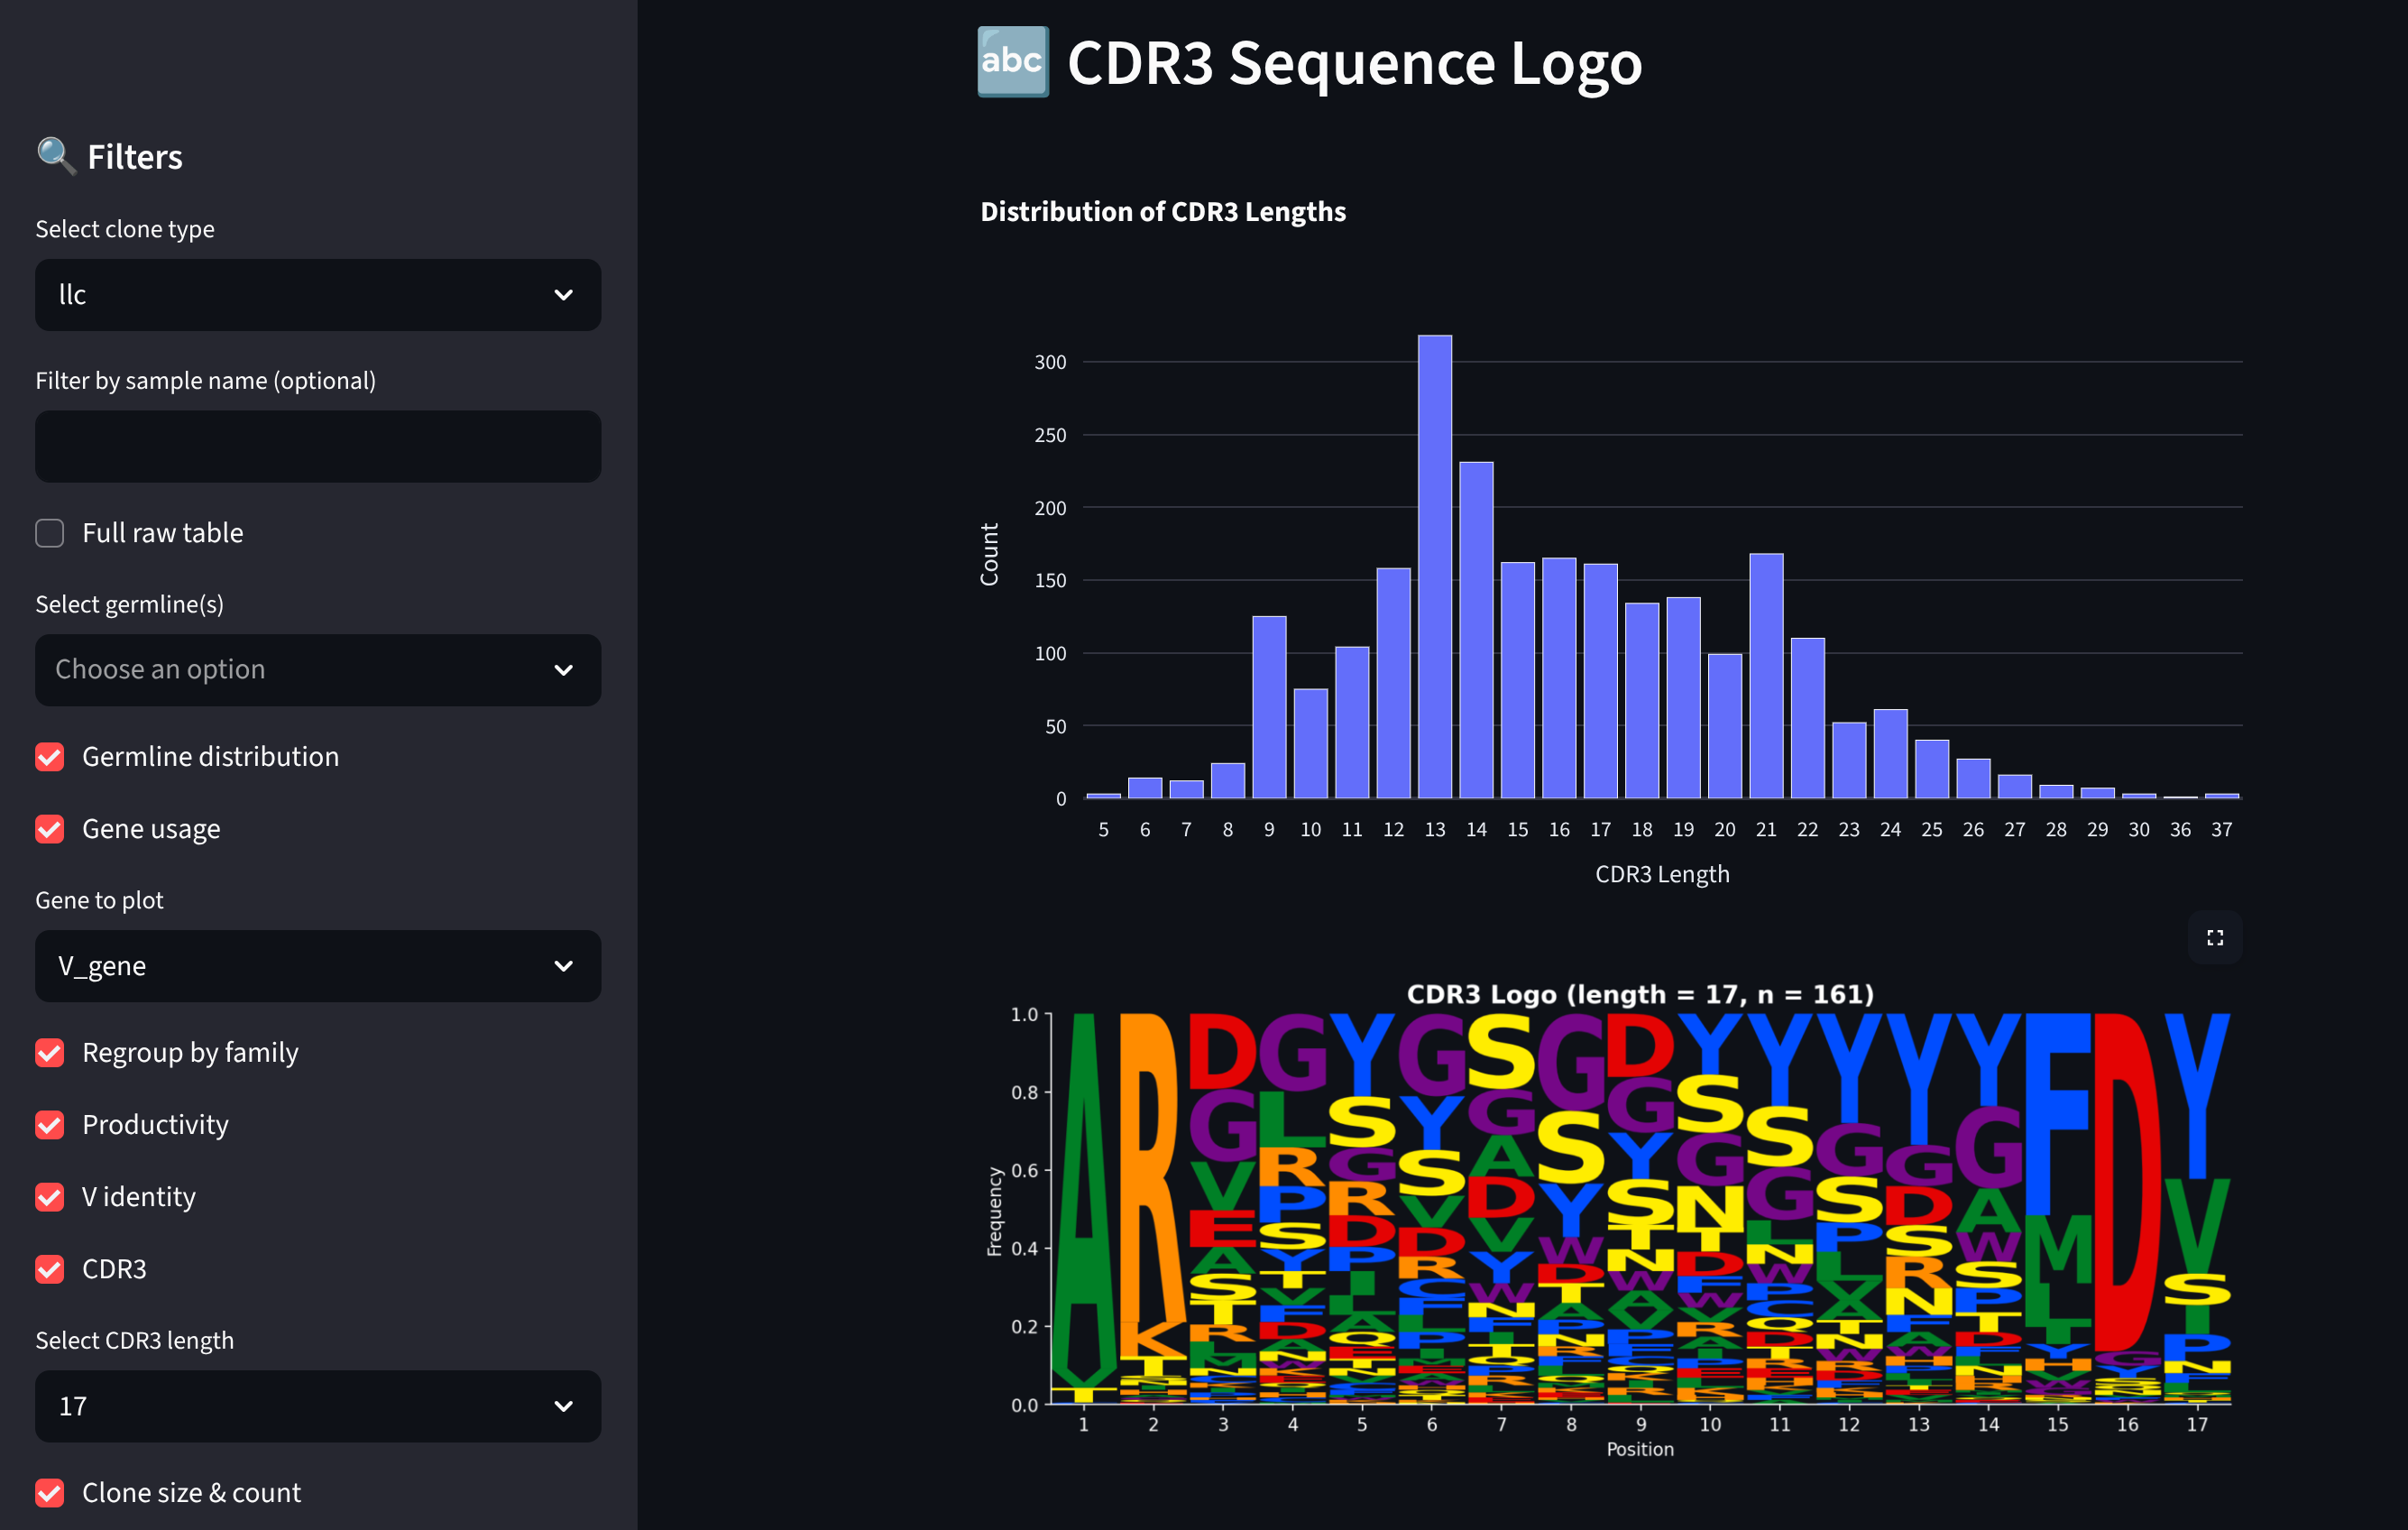
\includegraphics[width=1\textwidth]{images/vidjil_stat.png}
    \caption{
        Capture d'écran du tableau de bord pour la visualisation des statistiques des données de \textit{Vidjil}. 
        Exemple de la distribution de taille des séquences \gls{cdr}3 dans les \glspl{llc} et du logo des séquences 
        de taille 17.
        }
    \label{fig:vidjil-stat}
\end{figure}